\documentclass[12pt, a4paper]{article}

% Text languages
\usepackage[spanish, english, UKenglish, USenglish, american, british]{babel}

% Accents
\usepackage[latin1]{inputenc}

% Maths
\usepackage{mathtools}
\usepackage{amsmath,amsthm,amssymb}

% Double rows
\usepackage{multirow}

% Math-mode symbol & verbatim
\def\W#1#2{$#1{#2}$ &\tt\string#1\string{#2\string}}
\def\X#1{$#1$ &\tt\string#1}
\def\Y#1{$\big#1$ &\tt\string#1}
\def\Z#1{\tt\string#1}

% A non-floating table environment.
\makeatletter
\renewenvironment{table}%
   {\vskip\intextsep\parskip\z@
    \vbox\bgroup\centering\def\@captype{table}}%
   {\egroup\vskip\intextsep}
\makeatother

\DeclarePairedDelimiter\abs{\lvert}{\rvert}%
\DeclarePairedDelimiter\norm{\lVert}{\rVert}%

% Swap the definition of \abs* and \norm*, so that \abs
% and \norm resizes the size of the brackets, and the 
% starred version does not.
\makeatletter
\let\oldabs\abs
\def\abs{\@ifstar{\oldabs}{\oldabs*}}
%
\let\oldnorm\norm
\def\norm{\@ifstar{\oldnorm}{\oldnorm*}}
\makeatother

% C++
\usepackage{listings}
\usepackage{xcolor}
\lstset { %
	language = C++,
	backgroundcolor=\color{black!5}, % set backgroundcolor
    basicstyle=\footnotesize,% basic font setting
    tabsize=4, % tab space width
    showstringspaces=false, % don't mark spaces in strings
    %numbers=left, % display line numbers on the left
    commentstyle=\color{green}, % comment color
    keywordstyle=\color{blue}, % keyword color
    stringstyle=\color{red} % string color
}

% https://www.overleaf.com/learn/latex/Page_size_and_margins
\usepackage{geometry}
\topmargin = -23pt
\oddsidemargin = 13pt
\headheight = 12pt
\headsep = 25pt
\textheight = 674pt
\textwidth = 426pt
\marginparsep = 10pt
\marginparwidth = 50pt
\footskip = 30pt
\marginparpush = 5pt
\hoffset = 0pt
\voffset = 0pt
\paperwidth = 597pt
\paperheight = 845pt

% Hyperlinks
\usepackage{hyperref}

% Figure
\usepackage{graphicx}
\usepackage{caption}
\usepackage{subcaption}
\usepackage{etoc}
% Example
\newtheorem{exmp}{Example}[section]
% Algorithms
%\usepackage[]{algorithm2e}
%\usepackage{algorithm}% http://ctan.org/pkg/algorithm
%\usepackage{algpseudocode}% http://ctan.org/pkg/algorithmicx
\usepackage{algpseudocode}

\renewcommand{\thefootnote}{\arabic{footnote}} % 1, 2, 3... (la que hay por defecto)

\usepackage{titlesec}
\setcounter{secnumdepth}{5}

\titleformat{\paragraph}
{\normalfont\normalsize\bfseries}{\theparagraph}{1em}{}
\titlespacing*{\paragraph}
{0pt}{3.25ex plus 1ex minus .2ex}{1.5ex plus .2ex}

\usepackage{float}
%--------------------------------------------------------------------------
\title{PARALLELISM}
\author{Roger Vilaseca Darné and Xavier Martín Ballesteros\\
  \small UNIVERSITAT POLITÈCNICA DE CATALUNYA\\
}
\date{10th December 2018}

\begin{document}
% Images
\graphicspath{ {./lab2/images} }

%\maketitle

\begin{titlepage}
	\centering
%	{\scshape\LARGE UNIVERSITAT POLITÈCNICA DE CATALUNYA \par}
	\vspace{1cm}
	{\scshape\Large UNIVERSITAT POLITECNICA DE CATALUNYA\par}
	\vspace{1.5cm}
	{\huge\bfseries PARALLELISM\par}
	\vspace{2cm}
	{\Large\itshape \textbf{Lab 2: Brief tutorial on OpenMP programming model}\par}
	\vfill
	{\Large\itshape Roger Vilaseca Darne and Xavier Martin Ballesteros\break PAR4110\par}
	\vfill
	
\includegraphics[width=0.25\textwidth]{./images/UPC.png}\par\vspace{1cm}
	%supervised by\par
	%Dr.~Mark \textsc{Brown}

	\vfill

% Bottom of the page
	{\large 20th March 2019, Q1}
\end{titlepage}

%\abstract{Esto es una plantilla simple para un articulo en \LaTeX.}

%	*********************** ÍNDEX *********************
\setcounter{secnumdepth}{5}
\setcounter{tocdepth}{5}

\newpage
  \tableofcontents
\newpage

% Referència a una equació \ref{eq:area}).
% Referència a una secció \ref{sec:nada}
% Referència a una cita \cite{Cd94}.

\section{OpenMP questionnaire}

\subsection{Parallel regions}

\subsubsection{1.hello.c}

\textbf{1. How many times will you see the "Hello world!" message if the program is executed with "./1.hello"?}

If the program is executed with the given code, we see 24 times the message "Hello world!" because the number of threads has been set to 24. We can see it if we add the line \textbf{printf("\%d", omp\_get\_num\_threads());} in the code.

\hfill

\textbf{2. Without changing the program, how to make it to print 4 times the "Hello World!" message?}

We can change the number of threads to execute the code with the command \textbf{OMP\_NUM\_THREADS=4 ./1.hello}. This will execute the program 1.hello.c using only 4 threads. Thus, only 4 threads will output the "Hello World!" message.

\subsubsection{2.hello.c}

\textbf{1. Is the execution of the program correct? (i.e., prints a sequence of "(Thid) Hello (Thid)
world!" being Thid the thread identifier). If not, add a data sharing clause to make it correct?}

The execution of the program is not correct because there is no flow control inside the parallel region, so the 8 threads execute at the same time the code inside this region. Consequently, in the same line may appear "(Thread X) Hello (Thread Y) Hello..." without the second part of the print (Figure \ref{fig:bad_code}).

In order to make it correct, we have to add the \textbf{critical} clause as shown below. This clause specifies that code inside its region is executed by one thread at a time. The correct output is shown in Figure \ref{fig:good_code}.

\begin{figure}[H]
	\begin{lstlisting}
	#pragma omp parallel num_threads(8)
	#pragma omp critical
	{
	    id =omp_get_thread_num();
	    printf("(%d) Hello ",id);
	    printf("(%d) world!\n",id);
	}
	\end{lstlisting}
	\caption{Modified code of 2.hello.c.}
\end{figure}

\begin{figure}[H]
\begin{minipage}[b]{0.49\linewidth}

\begin{lstlisting}
	(0) Hello (0) world!
	(1) Hello (2) world!
	(4) Hello (6) Hello (6) world!
	(5) Hello (5) world!
	(2) Hello (7) Hello (5) world!
	(5) world!
	(6) world!
	(3) Hello (5) world!
\end{lstlisting}

\caption{Output of the original version of the code.}
\label{fig:bad_code}
\end{minipage}
\hspace{0.5cm}
\begin{minipage}[b]{0.46\linewidth}

\begin{lstlisting}
	(0) Hello (0) world!
	(4) Hello (4) world!
	(3) Hello (3) world!
	(6) Hello (6) world!
	(7) Hello (7) world!
	(1) Hello (1) world!
	(2) Hello (2) world!
	(5) Hello (5) world!
\end{lstlisting}

\caption{Output of the modified version of the code.}
\label{fig:good_code}
\end{minipage}
\end{figure}

\hfill

\textbf{2. Are the lines always printed in the same order? Why the messages sometimes appear intermixed? (Execute several times in order to see this).}

The lines are not always printed in the same order. This is because threads do not always arrive at the same moment in the critical region. Hence, in one execution it may happen that thread number 2 is the first to arrive to the critical part, so it will enter the first (preventing the other threads to enter the region) and printing correctly the first message, and in another execution thread number 2 may be the last one to enter the critical part, being the last to output the "Hello world!" message.

\subsubsection{3.how many.c}

\textbf{Assuming the OMP\_NUM\_THREADS variable is set to 8 with "export OMP\_NUM\_THREADS=8"}

\hfill

\textbf{1. How many "Hello world ..." lines are printed on the screen?}

Using 8 threads, the different "Hello world..." messages appear a total of 20 times.

\begin{itemize}
	\item Hello world from the first parallel (8)! $=>$ 8 times
	\item Hello world from the second parallel (2)! $=>$ 2 times
	\item Hello world from the second parallel (3)! $=>$ 3 times
	\item Hello world from the third parallel (4)! $=>$ 4 times
	\item Hello world from the fourth  parallel (3)! $=>$ 3 times
\end{itemize}

\hfill

\textbf{2. What does omp\_get\_num\_threads return when invoked outside and inside a parallel region?}

Outside the parallel region the function returns 1 because, as we are in a sequential part, there is only 1 thread executing the code.

There are several parallel regions (3 with \#pragma omp parallel and 1 with \#pragma omp parallel num\_threads(4)). The first region returns 8 threads, because we set the number of threads to use to 8.

The second region is inside the first loop of the main. Before calling \#pragma omp parallel, we set the number of threads to \textit{i}, which is the variable used in the for. This for is executed 2 times. In the first one, we set the number of threads to 2, so the value will be 2 threads. In the next loop iteration, the \textit{i} value is 3, so we will have 3 threads executing the parallel region.

In the next parallel region, we set with \textit{num\_threads(4)} the number of threads to execute the code, so the value in this region will be 4.

Finally, the last parallel region will be executed by 3 threads. Altough we previously set the number of threads to be 8, we changed later this value inside the loop. The last value was 3, so in this new region the value will still be 3.

\subsubsection{4.data\_sharing.c}

\textbf{1. Which is the value of variable x after the execution of each parallel region with different datasharing attributes (shared, private, firstprivate and reduction)? Is that the value you would expect? (Execute several times if necessary)}

The first datasharing attribute is \textbf{shared(x)}. This attribute makes variable \textit{x} to be shared by all the threads that are executing the code of this region. As we are modifying its value, it is possible that 2 threads read at the same time the \textit{x} value and later write in it their computed value. In this situation, the final value will not be the correct, as we have not added some values. This is what occurs sometimes. The value of this part was 107, similar as what we expected.

The second one is \textbf{private(x)}. This attribute specifies that each thread should have its own instance of the variable \textit{x}, initialised with a random value. Once we leave the parallel region, the \textit{x} value is again the one before executing this region. The value is 5, which is the expected value, because the print is done outside the parallel region and the value of \textit{x} was 5.

The next attribute, \textbf{firstprivate(x)}, is very similar to private. The main difference is that in this attribute the variable is initialized with the value of the variable, because it exists before the parallel construct. We print the value outside the parallel region, so the value is again 5.

The last attribute is \textbf{reduction(+:x)}. It specifies that variable \textit{x} that is private to each thread is the subject of a reduction operation at the end of the parallel region. It is initialized to the neutral value of the operation (sum in this case). The value is what we expected, 125 because the variable is private for each thread.

\begin{figure} [H]
	\begin{lstlisting}
	After first parallel (shared) x is: 107
	After second parallel (private) x is: 5
	After third  parallel (firstprivate) x is: 5
	After fourth parallel (reduction) x is: 125
	\end{lstlisting}
	\caption{Output of 4.data\_sharing.c.}
\end{figure}

\subsection{Loop parallelism}

\subsubsection{1.schedule.c}

\textbf{1. Which iterations of the loops are executed by each thread for each schedule kind?}

In \textbf{schedule(static)}, the iterations are divided by the number of threads. In this case, there will be 4 blocks of the same size (it may occur that the last block does not have the same size). The first block will correspond to the first thread, and successively. Thread 0 will execute block 0 (0-2 iterations), thread 1 will execute block 1 (3-5 iterations), thread 2 will execute block 2 (6-8 iterations) and thread 3 will execute block 4 (9-11 iterations).

We can enforce to create blocks of 2 iterations with \textbf{schedule(static, 2)}. Thread 0 will execute blocks 0 (0-1 iterations) and 4 (8-9 iterations). Thread 1 will execute 1 (2-3 iterations) and 5 (10-11 iterations). Thread 2, block 2 (4-5 iterations) and thread 3, block 3 (6-7 iterations).

The \textbf{schedule(dynamic, 2)} divides the iterations in blocks of 2 iterations, but it distributes the blocks in a different way than static. It gives the next block to execute to the first thread to end its work. This is a better solution, because it is possible that some thread has a lot of work in a block and it also has to execute another one. With dynamic, the other free threads will execute that second block, finishing the execution of the loop earlier. We cannot say which threads will execute each block, but we can ensure that for each block, the thread will execute two iterations of the loop.

The \textbf{schedule(guided, 2)} gives n/p iterations to the first loop, (n - n/p)/p iterations to the next loop and so on until blocks have 2 iterations. Then, it starts to work as a dynamic schedule.

\subsubsection{2.nowait.c}

\textbf{1. Which could be a possible sequence of printf when executing the program?}

In this code, two threads will execute the first loop while the other two threads execute the second loop. A possible sequence of prints would be the following:

\begin{figure}[H]
	\begin{lstlisting}
		Loop 1: thread (0) gets iteration 0
		Loop 1: thread (3) gets iteration 1
		Loop 2: thread (1) gets iteration 2
		Loop 2: thread (2) gets iteration 3
	\end{lstlisting}
	\caption{Possible output for 2.nowait.c.}
\end{figure}

\hfill

\textbf{2. How does the sequence of printf change if the nowait clause is removed from the first for
directive?}

Now, while two threads are executing the first loop, the other two will remain doing nothing. Once they end with the first loop, only 2 threads will enter in the second loop. As the schedule type is dynamic, we do not know which two threads will execute the for loops.

\begin{figure}[H]
	\begin{lstlisting}
	Loop 1: thread (0) gets iteration 0
	Loop 1: thread (1) gets iteration 1
	Loop 2: thread (0) gets iteration 2
	Loop 2: thread (1) gets iteration 3
	\end{lstlisting}
	\caption{Possible output for 2.nowait.c modified.}
\end{figure}

\hfill

\textbf{3. What would happen if dynamic is changed to static in the schedule in both loops? (keeping
the nowait clause)}

If we change it to static, threads 0 and 1 will execute the first and the second for loop because threads 2 and 3 will not receieve any work even though we have the nowait clauses.

\begin{figure}[H]
	\begin{lstlisting}
		Loop 1: thread (0) gets iteration 0
		Loop 1: thread (1) gets iteration 1
		Loop 2: thread (0) gets iteration 2
		Loop 2: thread (1) gets iteration 3
	\end{lstlisting}
	\caption{Output for 2.nowait.c modified.}
\end{figure}

\subsubsection{3.collapse.c}

\textbf{1. Which iterations of the loop are executed by each thread when the collapse clause is used?}

The \textbf{collapse} clause specifies how many loops in a nested loop should be collapsed into one large iteration space and divided according to the schedule clause. In this code, there is no schedule clause, so it will be treated as static.

\begin{figure}[H]
	\begin{lstlisting}
	Thread 0: 00, 01, 02, 03
	Thread 1: 04, 10, 11
	Thread 2: 12, 13, 14
	Thread 3: 20, 21, 22
	Thread 4: 23, 24, 30
	Thread 5: 31, 32, 33
	Thread 6: 34, 40, 41
	Thread 7: 42, 43, 44
	\end{lstlisting}
	\caption{Organization of the iterations in the threads. Being i the index for the first loop and j the index for the second loop, 00 means i = 0 and j = 0, 01 means i = 0 and j = 1...}
\end{figure}

\hfill

\textbf{2. Is the execution correct if the collapse clause is removed? Which clause (different than collapse) should be added to make it correct?}

The execution is not correct because some iterations are not executed. The main reason is because there are data racing conflicts with variable \textit{j}. To avoid this, we should make private the \textit{j} variable with \#pragma omp parallel for private(j).

\subsection{Synchronization}

\subsubsection{1.datarace.c}

\textbf{(execute several times before answering the questions)}

\hfill

\textbf{1. Is the program always executing correctly?}

The problem with this program is that everyone accesses the same variable to read and write.
This causes that some times two threads read x at the same time and each one executes its sum. Then, when writing the results one thread overwrites the result of the other thread.

\hfill

\textbf{2. Add two alternative directives to make it correct. Explain why they make the execution
correct.}

To solve this, we have proposed two solutions. The first one is very drastic because it turns the program into sequential:

\begin{figure}[H]
	\begin{lstlisting}
	#pragma omp parallel for schedule(dynamic,1) private(i) shared(x)
		for (i=0; i < N; i++) {
			#pragma omp atomic
			x++;
		}
	\end{lstlisting}
	
	\caption{Version 1 of the 1.datarace.c}
\end{figure}

As in each iteration of the loop each thread has to wait that the atomic region is free for the addition of the sum, threads wouldn't work in parallel.

The second solution consists of applying a reduction in x.

\begin{figure}[H]
	\begin{lstlisting}
	#pragma omp parallel for schedule(dynamic,1) private(i)
											     reduction(+:x)
		for (i=0; i < N; i++) {
			x++;
		}
	\end{lstlisting}
	
	\caption{Version 2 of the 1.datarace.c}
\end{figure}

Now, each thread will compute its own sum of x.
When all the threads finish, it will be computed the public x value using the precomputed sum of each thread.

\subsubsection{2.barrier.c}

\textbf{1. Can you predict the sequence of messages in this program? Do threads exit from the barrier
in any specific order?}

\hfill

In this program will be printed 4 lines saying the number of each thread and how long it will be doing a sleep.
Then when the sleep of each thread finishes, a line will be printed telling us which thread has been woken up.
Finally, 4 messages identified by each thread will appear, saying that everyone has already woken up.

We have been able to observe that the threads after the barrier do not appear in any specific order. However, before the barrier we can observe that the messages are ordered, because thread 0 will sleep less than 1, 2 and 3, thread 1 will sleep less than 2 and 3...

\subsubsection{3.ordered.c}

\textbf{1. Can you explain the order in which the "Outside" and "Inside" messages are printed?}

As the schedule clause is dynamic, the first thread created will be the first to execute the first iteration of the loop, and so on. As a consequence, the before messages appear in a messy way. However, in the case of the inside print, having "\#pragma omp ordered" forces the prints to be done in the same order in which iterations are distributed in the for, making the prints in an ordered way (thread X with i = 0 will print the first inside message even though it has not been the first to output the before message).

\hfill

\textbf{2. How can you ensure that a thread always executes two consecutive iterations in order during
the execution of the ordered part of the loop body?}

Adding the schedule(dynamic, 2) clause, each thread will have 2 consecutive iterations of the for. With the order clause, the iterations will be done in an ordered way and each thread will execute each time two consecutive iterations.

\subsection{Tasks}

\subsubsection{1.single.c}

\textbf{1. Can you explain why all threads contribute to the execution of instances of the single worksharing construct? Why are those instances appear to be executed in bursts?}

Thanks to the \textbf{single} clause only 1 thread executes each iteration of the loop, and thanks to the \textbf{nowait} clause, the other threads do not have to wait until the iteration ends to continue with the other iterations.

The 4 threads distribute the first 4 iterations. They print a message and remain sleeping during 1 second. Then, they distribute again the 4 next iterations, and so on. As a consequence, we see the messages in bursts.

\subsubsection{2.fibtasks.c}

\textbf{1. Why all tasks are created and executed by the same thread? In other words, why the program is not executing in parallel?}

The program has 0 parallel regions, so only 1 thread is executing the code. Thus, only 1 thread creates tasks and executes them.

\hfill

\textbf{2. Modify the code so that the program correctly executes in parallel, returning the same answer that the sequential execution would return.}

\begin{figure}[H]
	\begin{lstlisting}
	#pragma omp parallel
    #pragma omp single
    while (p != NULL) {
          printf("Thread %d creating task that will compute %d\n",
          		  omp_get_thread_num(), p->data);
          #pragma omp task firstprivate(p)
          processwork(p);
          p = p->next;
    }
	\end{lstlisting}
	\caption{Modified version of 2.fibtasks.c.}
\end{figure}


First of all we add "\#pragma omp parallel" over the loop in order to make the execution parallel. However, this feature make that each thread creates all the tasks, giving us a wrong result.
The solution has been adding a "\#pragma omp simple" between the parallel and the while, and adding the clause firstprivate(p) in the task creation.
This makes that only the first thread creates all the tasks and each task has copy of the p value. Afterwards, all the threads can compute individually each task as soon as are created and the threads are free.

\subsubsection{3.synchtasks.c}

\textbf{1. Draw the task dependence graph that is specified in this program}

The \textbf{depend} clause establish dependences, only between tasks, on the scheduling of tasks. There are different types of dependence:

\begin{itemize}
	\item \textbf{in}: The task has to wait until all previously generated sibling tasks that reference at least one of the list items in an \textit{out} or \textit{inout} list end their execution.
	\item \textbf{out} and \textbf{inout}: The task has to wait untill all previously generated sibling tasks that reference at least one of the list items in an \textit{in}, \textit{out} or \textit{inout} list end their execution.
\end{itemize}

In the given code, the first task has an \textbf{out} depende type, with only the variable \textit{a} in its list. As there are no previously generated sibling tasks, this first task is not dependent of any task. Tasks 2 and 3 are not dependent of any previously generated sibling task because, although there exist some previously sibling tasks, none of them has variables \textit{b} or \textit{c} in its lists.

On the other hand, task 4 has an \textbf{in} dependence type with variables \textit{a} and \textit{b} and an \textbf{out} dependence type with variable \textit{d}. Thus, this task will have to wait until tasks 1 and 2 end their execution.

Finally, task 5 has an \textbf{in} dependence type with variables \textit{c} and \textit{d}. This task will depend from tasks 3 and 4. Hence, the task dependence graph is the following:

\begin{figure}[H]
  \centering
  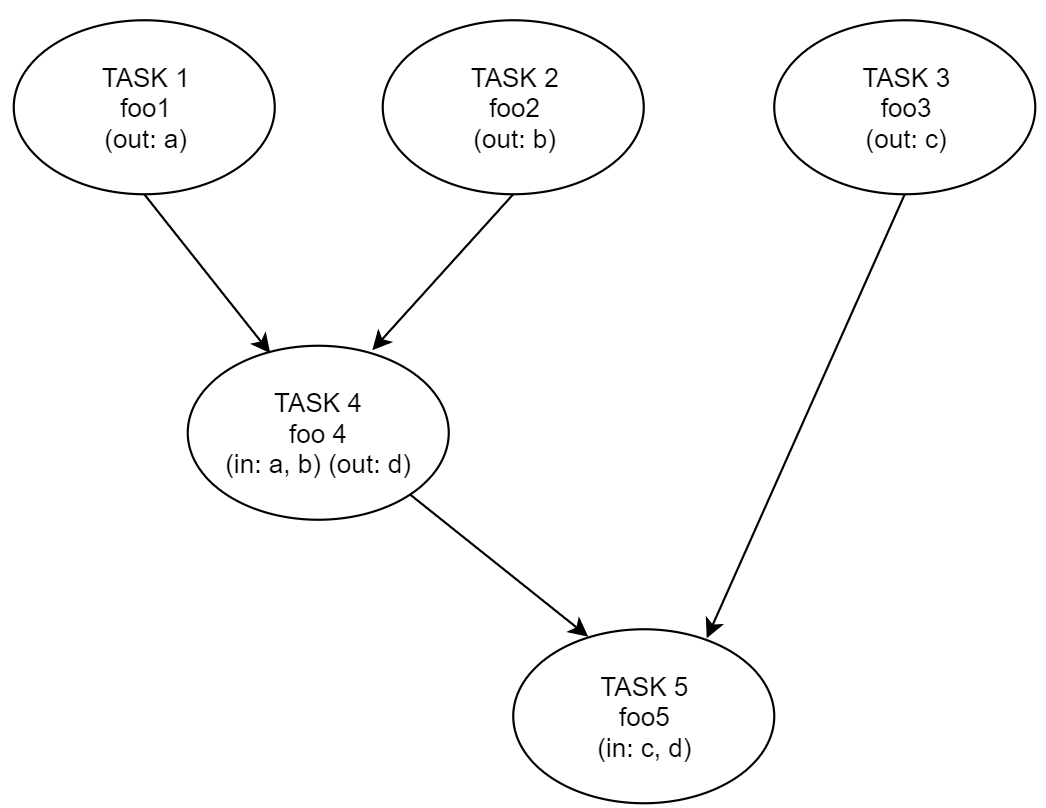
\includegraphics[scale=0.5]{./images/synchtasks}
  \caption{Task dependency graph of code 3.synchtasks.c.}
  \label{Task dependency graph of code 3.synchtasks.c.}
\end{figure}

\hfill

\textbf{2. Rewrite the program using only taskwait as task synchronisation mechanism (no depend clauses allowed)}

The \textbf{taskwait} construct makes a task wait until the completion of its child tasks. The new version of the code is shown below. Task 4 will wait until tasks 1 and 2 end their execution and task 5 will wait until the completition of tasks 3 and 4. Doing this we recreated the task dependency graph of Figure \ref{Task dependency graph of code 3.synchtasks.c.} without using the \textbf{depend} clause.

The first problem we have seen is that task 3 cannot be executed at the same time than tasks 1 and 2. Otherwise, task 4 would have to wait until tasks 1, 2 and 3 end their execution altough it does not depend from task 3. The second problem is that with this code, we are not able to create the 5 tasks at the same time. Tasks 1, 2 and 4 will be created first. Then tasks 3 and 5.

\begin{figure}[H]
	\begin{lstlisting}
	printf("Creating task foo1\n");
	#pragma omp task
	foo1();
	
	printf("Creating task foo2\n");
	#pragma omp task
	foo2();
	
	printf("Creating task foo4\n");
	#pragma omp taskwait
	foo4();

	printf("Creating task foo3\n");
	#pragma omp task
	foo3();
	
	printf("Creating task foo5\n");
	#pragma omp taskwait
	foo5();
	\end{lstlisting}
	
	\caption{Modified version of the given code.}
\end{figure}

Figures \ref{fig:original_code} and \ref{fig:modified_code} show the output when executing the two versions of the code. We can see clearly the differences between one and the other explained before.

\begin{figure}[H]
\begin{minipage}[b]{0.47\linewidth}

\begin{lstlisting}
	Creating task foo1
	Creating task foo2
	Creating task foo3
	Creating task foo4
	Creating task foo5
	Starting function foo3
	Starting function foo1
	Starting function foo2
	Terminating function foo1
	Terminating function foo2
	Starting function foo4
	Terminating function foo4
	Terminating function foo3
	Starting function foo5
	Terminating function foo5
\end{lstlisting}

\caption{Output of the original version of the code.}
\label{fig:original_code}
\end{minipage}
\hspace{0.5cm}
\begin{minipage}[b]{0.48\linewidth}

\begin{lstlisting}
	Creating task foo1
	Creating task foo2
	Creating task foo4
	Starting function foo2
	Starting function foo1
	Terminating function foo2
	Terminating function foo1
	Starting function foo4
	Terminating function foo4
	Creating task foo3
	Creating task foo5
	Starting function foo3
	Terminating function foo3
	Starting function foo5
	Terminating function foo5
\end{lstlisting}

\caption{Output of the modified version of the code.}
\label{fig:modified_code}
\end{minipage}
\end{figure}

\subsubsection{4.taskloop.c}

\textbf{1. Find out how many tasks and how many iterations each task execute when using the grainsize and num tasks clause in a taskloop. You will probably have to execute the program several times in order to have a clear answer to this question.}

The \textbf{grainsize(grain-size)} clause controls how many loop iterations are assigned to each created task. The number of loop iterations assigned to each created task is greater than or equal to the minimum of the value of grain-size and the total number of iterations.

We though that when using the \textbf{grainsize(5)} clause there will be created 3 tasks, the first two executing 5 iterations and the other one 2. In reality, there are only 2 tasks created, each one executing 6 iterations. This is because the number 5 does not mean that each task has 5 iterations but a minimum of 5.

The \textbf{num\_tasks(num-tasks)} clause creates as many tasks as the minimum of num-tasks and the number of loop iterations.

There are 5 tasks created. The first two execute 3 iterations of the loop whereas the other 3 execute only 2.

\begin{figure}[H]
	\begin{lstlisting}
	Going to distribute 12 iterations with grainsize(5) ...
	Loop 1: (1) gets iteration 0
	Loop 1: (1) gets iteration 1
	Loop 1: (1) gets iteration 2
	Loop 1: (1) gets iteration 3
	Loop 1: (2) gets iteration 6
	Loop 1: (2) gets iteration 7
	Loop 1: (2) gets iteration 8
	Loop 1: (2) gets iteration 9
	Loop 1: (2) gets iteration 10
	Loop 1: (2) gets iteration 11
	Loop 1: (1) gets iteration 4
	Loop 1: (1) gets iteration 5
	Going to distribute 12 iterations with num_tasks(5) ...
	Loop 2: (2) gets iteration 0
	Loop 2: (2) gets iteration 1
	Loop 2: (1) gets iteration 6
	Loop 2: (1) gets iteration 7
	Loop 2: (0) gets iteration 10
	Loop 2: (0) gets iteration 11
	Loop 2: (1) gets iteration 8
	Loop 2: (1) gets iteration 9
	Loop 2: (2) gets iteration 2
	Loop 2: (3) gets iteration 3
	Loop 2: (3) gets iteration 4
	Loop 2: (3) gets iteration 5
	\end{lstlisting}
	
	\caption{Ouput of the code without the nogroup clause.}
\end{figure}

\hfill

\textbf{2. What does occur if the nogroup clause in the first taskloop is uncommented?}

The \textbf{taskloop} clause implicitly generates a \textbf{taskgroup} region that encloses it. In this region there is a barrier at the end, so the second loop will not be executed until the first one terminates. The \textbf{nogroup} clause removes the \textbf{taskgroup} region.

With the \textbf{nogroup} clause, the second loop can be executed at the same time than the first loop.

Now, there are created the same number of tasks, and each one does the same itreations than in the previous question. However, while two threads execute the first loop, the other two threads will execute the 5 tasks of the second loop (Figure \ref{Ouput 1 of the code with the nogroup clause.}), unless one of the two threads of the first loop end before the second loop terminates. In this situation, this thread will also execute tasks of the second loop (Figure \ref{Ouput 2 of the code with the nogroup clause.}).

\begin{figure}[H]
	\begin{lstlisting}
	Going to distribute 12 iterations with grainsize(5) ...
	Going to distribute 12 iterations with num_tasks(5) ...
	Loop 1: (1) gets iteration 0
	Loop 1: (1) gets iteration 1
	Loop 1: (2) gets iteration 6
	Loop 1: (2) gets iteration 7
	Loop 1: (2) gets iteration 8
	Loop 1: (1) gets iteration 2
	Loop 2: (0) gets iteration 10
	Loop 2: (0) gets iteration 11
	Loop 2: (0) gets iteration 8
	Loop 2: (3) gets iteration 0
	Loop 2: (3) gets iteration 1
	Loop 2: (3) gets iteration 2
	Loop 2: (3) gets iteration 3
	Loop 2: (3) gets iteration 4
	Loop 2: (3) gets iteration 5
	Loop 2: (3) gets iteration 6
	Loop 2: (3) gets iteration 7
	Loop 1: (1) gets iteration 3
	Loop 1: (1) gets iteration 4
	Loop 1: (1) gets iteration 5
	Loop 2: (0) gets iteration 9
	Loop 1: (2) gets iteration 9
	Loop 1: (2) gets iteration 10
	Loop 1: (2) gets iteration 11
	\end{lstlisting}
	
	\caption{Ouput 1 of the code with the nogroup clause.}
	\label{Ouput 1 of the code with the nogroup clause.}
\end{figure}

\begin{figure}[H]
	\begin{lstlisting}
	Going to distribute 12 iterations with grainsize(5) ...
	Going to distribute 12 iterations with num_tasks(5) ...
	Loop 1: (2) gets iteration 0
	Loop 1: (2) gets iteration 1
	Loop 1: (2) gets iteration 2
	Loop 1: (2) gets iteration 3
	Loop 1: (2) gets iteration 4
	Loop 1: (2) gets iteration 5
	Loop 1: (1) gets iteration 6
	Loop 1: (1) gets iteration 7
	Loop 1: (1) gets iteration 8
	Loop 2: (0) gets iteration 10
	Loop 2: (3) gets iteration 3
	Loop 1: (1) gets iteration 9
	Loop 1: (1) gets iteration 10
	Loop 1: (1) gets iteration 11
	Loop 2: (0) gets iteration 11
	Loop 2: (0) gets iteration 8
	Loop 2: (0) gets iteration 9
	Loop 2: (3) gets iteration 4
	Loop 2: (3) gets iteration 5
	Loop 2: (1) gets iteration 6
	Loop 2: (1) gets iteration 7
	Loop 2: (2) gets iteration 0
	Loop 2: (2) gets iteration 1
	Loop 2: (2) gets iteration 2
	\end{lstlisting}
	
	\caption{Ouput 2 of the code with the nogroup clause.}
	\label{Ouput 2 of the code with the nogroup clause.}
\end{figure}

\section{Observing overheads}

\subsection{Synchronisation overheads}

In this section we have different ways of computing the pi number, each using a different synchronization method for the sum variable. Although all the codes compute the correct value of the pi number, some of them are slower than the others. We have also used the \textit{Paraver} to see the synchronization between threads.

We will see an improvement in the usage of the potential parallelism, in decreasing the execution time and the overheads. As we achieved to reduce the overheads in the parallel region, we will see that the traces in the \textit{Paraver} will end up being very small in the parallel region.

\subsubsection{pi\_sequential.c}

The code in \textit{pi\_sequential.c} makes no profit about the potential parallelism it has to compute the pi value. It only executes the code in sequential. The values we obtained are shown below.

\begin{figure}[H]
	\begin{lstlisting}
	Wall clock execution time  = 1.793329954 seconds
	Value of pi = 3.1415926536		
	\end{lstlisting}
	\caption{Output of pi\_sequential.}
\end{figure}

\begin{figure}[H]
  \centering
  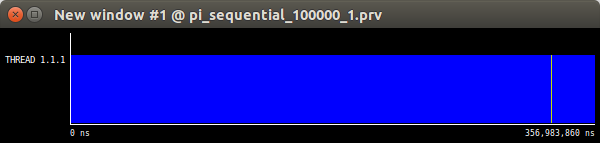
\includegraphics[scale=0.5]{./images/pi_sequential}
  \caption{Execution flow of pi\_sequential.c.}
  \label{pi_sequential}
\end{figure}

The execution time value will be very useful to do comparisons with the different synchronization methods.

\subsubsection{pi\_omp\_critical.c}

The code given in \textit{pi\_omp\_critical.c} makes use of the \textbf{critical} method. Thus, only 1 thread can execute at the same time the critical region. Every time one thread enters the region it executes one synchronization operation (\textit{omp\_set\_lock(...))} and each time any threads leaves the region it executes another syncrhonization operation (\textit{omp\_unset\_lock(...))}. Hence, the total number of synchronization operations is $2 * num\_steps $.

\begin{figure}[H]
	\begin{lstlisting}
	#pragma omp parallel private(x) num_threads(num_threads)
    {
        #pragma omp for 
        for (long int i=0; i<num_steps; ++i) {
            x = (i+0.5)*step;
            #pragma omp critical 
	    	sum += 4.0/(1.0+x*x);
        }
    }
	\end{lstlisting}
	
	\caption{Parallel code (pi\_omp\_critical).}
\end{figure}

Using the critical method, the execution time of this version with 1 thread takes around 2.5s more than the sequential execution. We think that this is because each time we want to update the sum variable we have to \textit{omp\_set\_lock(critical\_region)} and \textit{ omp\_unset\_lock(critical\_region)}. These two calls with a big number of iterations ends up being a significant overhead. Figure \ref{pi_omp_critical_1_zoom} shows the synchronization overheads.

\begin{figure}[H]
	\begin{lstlisting}
	Total execution time: 4.319360s
	Number pi after 100000000 iterations = 3.141592653590426		
	\end{lstlisting}
	\caption{Output of pi\_omp\_critical with 1 thread.}
\end{figure}

\begin{figure}[H]
  \centering
  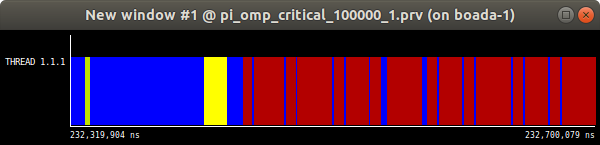
\includegraphics[scale=0.5]{./images/pi_omp_critical_1_zoom}
  \caption{Execution flow of pi\_omp\_critical.c with 1 thread (zoomed).}
  \label{pi_omp_critical_1_zoom}
\end{figure}

From 2 threads, the execution time increases a lot because if we execute the code with only 1 thread, this thread does not have to synchronizate with any other thread, so when it ends one iteration it can start the next one. However, if we have more than one thread, the threads have to synchronizate in order that only 1 thread executes the critical region. These synchronizations increase a lot the overhead. Thus, from 2 threads, the execution time increases around 30s. Figures \ref{piompcritical4} and \ref{piompcritical8} show the output of the execution with 4 and 8 threads and figures \ref{pi_omp_critical_4_zoom} and \ref{pi_omp_critical_8_zoom} shows the synchronization flow operations.

\begin{figure}[H]
	\begin{lstlisting}
	Total execution time: 38.100659s
	Number pi after 100000000 iterations = 3.141592653590203		
	\end{lstlisting}
	\caption{Output of pi\_omp\_critical with 4 threads.}
	\label{piompcritical4}
\end{figure}

\begin{figure}[H]
  \centering
  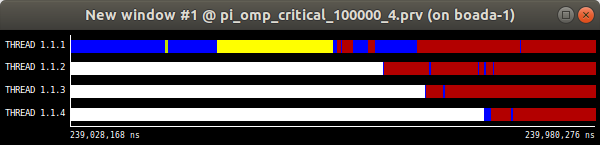
\includegraphics[scale=0.5]{./images/pi_omp_critical_4_zoom}
  \caption{Execution flow of pi\_omp\_critical.c with 4 threads (zoomed).}
  \label{pi_omp_critical_4_zoom}
\end{figure}

\begin{figure}[H]
	\begin{lstlisting}
	Total execution time: 34.410379s
	Number pi after 100000000 iterations = 3.141592653589771		
	\end{lstlisting}
	\caption{Output of pi\_omp\_critical with 8 threads.}
	\label{piompcritical8}
\end{figure}

\begin{figure}[H]
  \centering
  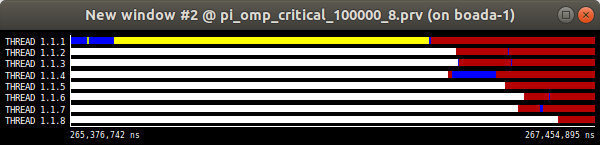
\includegraphics[scale=0.5]{./images/pi_omp_critical_8_zoom}
  \caption{Execution flow of pi\_omp\_critical.c with 8 threads (zoomed).}
  \label{pi_omp_critical_8_zoom}
\end{figure}

\subsubsection{pi\_omp\_atomic.c}

This code can be found in \textit{pi\_omp\_atomic.c}. It uses the \textbf{atomic} method. With this, only 1 thread will be able to execute the sum part although the other threads can compute $4.0/(1.0+x*x)$ in parallel. As we have to lock and unlock that region, the total number of synchronization operations is again $2 * num\_steps$.

\begin{figure}[H]
	\begin{lstlisting}
	#pragma omp parallel private(x) num_threads(num_threads)
    {
        #pragma omp for 
        for (long int i=0; i<num_steps; ++i) {
            x = (i+0.5)*step;
            #pragma omp atomic 
	    	sum += 4.0/(1.0+x*x);
        }
    }
	\end{lstlisting}
	
	\caption{Parallel code (pi\_omp\_atomic).}
\end{figure}

The execution time of the code using the atomic clause and 1 thread does not increase with respect to the sequential execution. We think that this happens because the overhead of this clause is smaller than the critical one (in figure \ref{pi_omp_atomic_1_zoom} we cannot see any syncrhonization operation in red). Moreover, when it ends the execution of one iteration it does not have to wait until another thread ends its execution.

\begin{figure}[H]
	\begin{lstlisting}
	Total execution time: 1.794664s
	Number pi after 100000000 iterations = 3.141592653590426		
	\end{lstlisting}
	\caption{Output of pi\_omp\_atomic with 1 thread.}
\end{figure}

\begin{figure}[H]
  \centering
  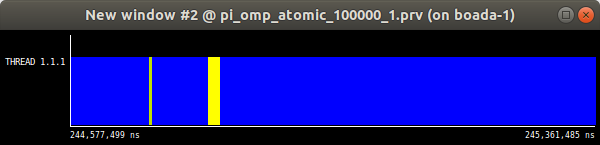
\includegraphics[scale=0.5]{./images/pi_omp_atomic_1_zoom}
  \caption{Execution flow of pi\_omp\_atomic.c with 1 thread (zoomed).}
  \label{pi_omp_atomic_1_zoom}
\end{figure}

With 4 and 8 threads, the execution time increases a little beacause in each iteration, threads must wait the variable sum to be free. This makes threads to synchronize between them. Consequently, there is a small overhead. Nevertheless, these overheads are smaller than the critical ones because they only lock the region where we read, operate and write the variable sum (in the critical version, it locked the region where we read, operate and write the variable sum and compute the operation $4.0/(1.0+x*x)$).

\begin{figure}[H]
	\begin{lstlisting}
	Total execution time: 6.201648s
	Number pi after 100000000 iterations = 3.141592653590225			
	\end{lstlisting}
	\caption{Output of pi\_omp\_atomic with 4 threads.}
	\label{piompatomic4}
\end{figure}

\begin{figure}[H]
  \centering
  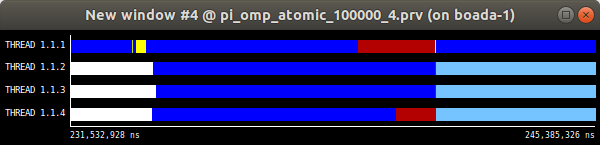
\includegraphics[scale=0.5]{./images/pi_omp_atomic_4_zoom}
  \caption{Execution flow of pi\_omp\_atomic.c with 4 threads (zoomed).}
  \label{pi_omp_atomic_4_zoom}
\end{figure}

\begin{figure}[H]
	\begin{lstlisting}
	Total execution time: 6.910445s
	Number pi after 100000000 iterations = 3.141592653589742
	\end{lstlisting}
	\caption{Output of pi\_omp\_atomic with 8 threads.}
	\label{piompatomic8}
\end{figure}

\begin{figure}[H]
  \centering
  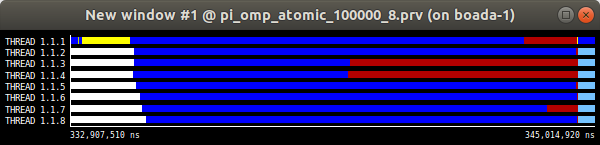
\includegraphics[scale=0.5]{./images/pi_omp_atomic_8_zoom}
  \caption{Execution flow of pi\_omp\_atomic.c with 8 threads (zoomed).}
  \label{pi_omp_atomic_8_zoom}
\end{figure}

Figures \ref{piompatomic4} and \ref{piompatomic8} show a big decrease of the execution time with respect to the critical times (34 and 38 to 6 and 7 approximately).

We discussed a lot about the results in \textit{Paraver} (figures \ref{pi_omp_atomic_4_zoom} and \ref{pi_omp_atomic_8_zoom}) because it was not what we think it would appear. What we thinked was that there should be small regions in red (synchronization), regions where only one thread would execute the atomic region while the others wait, but there is only 1 big line in the end (barrier). Our conclusion with this is that \textit{Paraver} cannot make enough zoom to see those small lines, even though they are there.

\subsubsection{pi\_omp\_reduction.c}

The code with the \textbf{reduction} clause can be found in \textit{pi\_omp\_reduction.c}. This new clause will create its own private sum variable initialized to 0 (neutral value of the sum operation). In the end, threads will have to syncrhonize to update securely the public sum variable. Thus, the total number of synchronization will be $2 * \#threads$.

\begin{figure}[H]
	\begin{lstlisting}
	#pragma omp parallel private(x) num_threads(num_threads)
								    reduction(+:sum)
    {
        #pragma omp for 
        for (long int i=0; i<num_steps; ++i) {
            x = (i+0.5)*step;
	    	sum += 4.0/(1.0+x*x);
        }
    }

	\end{lstlisting}
	
	\caption{Parallel code (pi\_omp\_reduction).}
\end{figure}

In this case, the execution time with 1 thread gets worse than the sequential time (+0.3s) because it has to create 1 new private variable (sum) and this generates overhead. In the end, the thread has to wait to synchronize with the other threads and write into the public sum variable. As there is only 1 thread, this overhead will be insignificant. We can see this overhead at the end of Figure \ref{pi_omp_reduction_1_zoom}.

\begin{figure}[H]
	\begin{lstlisting}
	Total execution time: 1.831957s
	Number pi after 100000000 iterations = 3.141592653590426		
	\end{lstlisting}
	\caption{Output of pi\_omp\_reduction with 1 thread.}
	\label{piompreduction1}
\end{figure}

\begin{figure}[H]
  \centering
  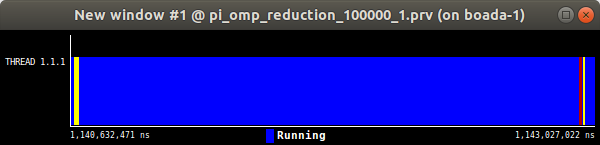
\includegraphics[scale=0.5]{./images/pi_omp_reduction_1_zoom}
  \caption{Execution flow of pi\_omp\_reduction.c with 1 thread (zoomed).}
  \label{pi_omp_reduction_1_zoom}
\end{figure}

Using 4 and 8 threads we observe a great improvement. In this version, we make profit of the potential parallelism of the code because each thread will have its own variable sum, making possible that any thread has to remain blocked during the for execution. They will only need synchronization at the end of the for loop to sum all the private sum variables with the public sum variable. Outputs are shown in figures \ref{piompreduction4} and \ref{piompreduction8}.

\begin{figure}[H]
	\begin{lstlisting}
	Total execution time: 0.478957s
	Number pi after 100000000 iterations = 3.141592653589683			
	\end{lstlisting}
	\caption{Output of pi\_omp\_reduction with 4 threads.}
	\label{piompreduction4}
\end{figure}

\begin{figure}[H]
  \centering
  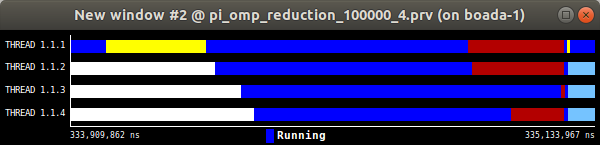
\includegraphics[scale=0.5]{./images/pi_omp_reduction_4_zoom}
  \caption{Execution flow of pi\_omp\_reduction.c with 4 threads (zoomed).}
  \label{pi_omp_reduction_4_zoom}
\end{figure}

\begin{figure}[H]
	\begin{lstlisting}
	Total execution time: 0.261439s
	Number pi after 100000000 iterations = 3.141592653589815
	\end{lstlisting}
	\caption{Output of pi\_omp\_reduction with 8 threads.}
	\label{piompreduction8}
\end{figure}

\begin{figure}[H]
  \centering
  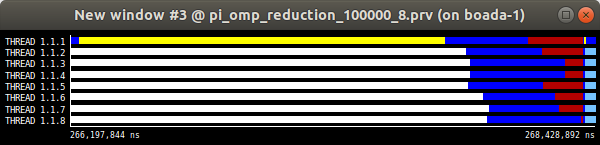
\includegraphics[scale=0.5]{./images/pi_omp_reduction_8_zoom}
  \caption{Execution flow of pi\_omp\_reduction.c with 8 threads (zoomed).}
  \label{pi_omp_reduction_8_zoom}
\end{figure}

In figures \ref{pi_omp_reduction_4_zoom} and \ref{pi_omp_reduction_8_zoom} we can see what we said before. During the execution of the loop, there is no synchronization (continuous blue line). However, at the end of the loop there is a synchronization operation to update correctly the public sum variable.

\subsubsection{pi\_omp\_sumlocal.c}

The code can be found in \textit{pi\_omp\_sumlocal}. This version simulates the reduction clause without using it. To achieve it, it is created a public variable (sumlocal) that is privatized inside the parallel region with the initial value. With this, each thread will have its own sumlocal variable. They will only have to syncrhonize after the for loop, when updating the sum variable. Hence, the total number of syncrhonization operations is $2 * \#threads$.

\begin{figure}[H]
	\begin{lstlisting}
	double sumlocal = 0.0;
	#pragma omp parallel private(x) firstprivate(sumlocal)
									num_threads(num_threads)
    {
        #pragma omp for 
        for (long int i=0; i<num_steps; ++i) {
            x = (i+0.5)*step;
            sumlocal += 4.0/(1.0+x*x);
        }
        #pragma omp critical 
		sum += sumlocal;
    }


	\end{lstlisting}
	
	\caption{Parallel code (pi\_omp\_sumlocal).}
\end{figure}

The outputs and execution flows are the same than in the reduction code. This reinforce what we said about that this and the reduction codes are the same using different clauses.

\begin{figure}[H]
	\begin{lstlisting}
	Total execution time: 1.832351s
	Number pi after 100000000 iterations = 3.141592653590426		
	\end{lstlisting}
	\caption{Output of pi\_omp\_sumlocal with 1 thread.}
\end{figure}

\begin{figure}[H]
  \centering
  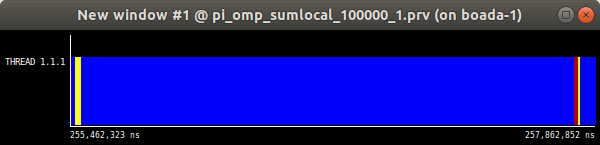
\includegraphics[scale=0.5]{./images/pi_omp_sumlocal_1_zoom}
  \caption{Execution flow of pi\_omp\_sumlocal.c with 1 thread (zoomed).}
  \label{pi_omp_sumlocal_1_zoom}
\end{figure}

\begin{figure}[H]
	\begin{lstlisting}
	Total execution time: 0.482865s
	Number pi after 100000000 iterations = 3.141592653589683					
	\end{lstlisting}
	\caption{Output of pi\_omp\_sumlocal with 4 threads.}
\end{figure}

\begin{figure}[H]
  \centering
  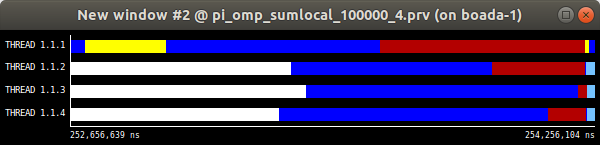
\includegraphics[scale=0.5]{./images/pi_omp_sumlocal_4_zoom}
  \caption{Execution flow of pi\_omp\_sumlocal.c with 4 thread (zoomed).}
  \label{pi_omp_sumlocal_4_zoom}
\end{figure}

\begin{figure}[H]
	\begin{lstlisting}
	Total execution time: 0.261369s
	Number pi after 100000000 iterations = 3.141592653589815		
	\end{lstlisting}
	\caption{Output of pi\_omp\_sumlocal with 8 threads.}
\end{figure}

\begin{figure}[H]
  \centering
  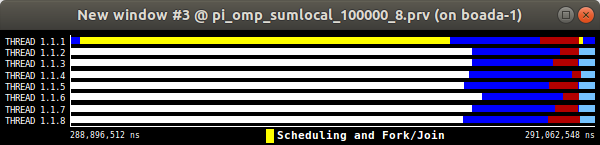
\includegraphics[scale=0.5]{./images/pi_omp_sumlocal_8_zoom}
  \caption{Execution flow of pi\_omp\_sumlocal.c with 8 thread (zoomed).}
  \label{pi_omp_sumlocal_8_zoom}
\end{figure}

\subsection{Thread creation and termination}

Code \textit{pi\_omp\_parallel.c} is used to calculate the thread creation and termination overhead. To do this, the code has 2 parts which computes the same value (pi), one sequential and the other parallel. The tricky part is that in the parallel region only 1 thread executes the code, so it takes the same time than in the sequential part. As a result, the difference between the sequential and the parallel regions will only be caused by the overheads.

The order of magnitud of the overhead generated in the threads creation is in microseconds. We can see it clearly in Figure \ref{piompparallel} because the first print is a message with the order of magnitude.

\begin{figure}[H]
	\begin{lstlisting}
	All overheads expressed in microseconds
	Nthr    Overhead        Overhead per thread
	2       2.0023          1.0011
	3       1.6780          0.5593
	4       1.7134          0.4284
	5       1.7847          0.3569
	6       1.8046          0.3008
	7       1.7323          0.2475
	8       1.7549          0.2194
	9       2.2797          0.2533
	10      2.3004          0.2300
	11      2.3724          0.2157
	12      2.4019          0.2002
	13      2.4509          0.1885
	14      2.5782          0.1842
	15      2.7435          0.1829
	16      2.7500          0.1719
	17      2.8480          0.1675
	18      2.8822          0.1601
	19      2.8254          0.1487
	20      2.9179          0.1459
	21      2.9622          0.1411
	22      3.0387          0.1381
	23      3.0811          0.1340
	24      3.7695          0.1571
	\end{lstlisting}
	\caption{Output of pi\_omp\_parallel.c (execution in queue).}
	\label{piompparallel}
\end{figure}

On the one hand, we see that the bigger the number of threads used, the bigger the overhead. This is because we have to create and terminate more threads.

On the other hand, the overhead per thread decreases as we increase the number of threads. We think that this may happen because the total time to initialize a parallel region is much greater than the total time to initialize a thread. As a consequence, if we use more threads, the creation and termination overheads are not significant with respect to the time to initialize the parallel region, so these two operations will not increase a lot the value of the total overhead and the overhead per thread will decrease.

\subsection{Task creation and synchronization}

In this section, we studied the overhead when creating tasks and synchronizing them.

The order of magnitude is also in microsecond. It is shown in the first line of Figure \ref{piomptasks}. The execution was using 10 tasks and 1 thread. If we compute $T_{par} - T_{seq}$, we only have the overhead of the creation (\textbf{task)} and synchronization (\textbf{taskwait}) of the tasks.

\begin{figure}[H]
\begin{lstlisting}
	All overheads expressed in microseconds
	Ntasks  Overhead        Overhead per task
	2       0.2318          0.1159
	4       0.5196          0.1299
	6       0.7690          0.1282
	8       1.0167          0.1271
	10      1.2827          0.1283
	12      1.5125          0.1260
	14      1.7640          0.1260
	16      2.0038          0.1252
	18      2.2672          0.1260
	20      2.5160          0.1258
	22      2.7558          0.1253
	24      3.0027          0.1251
	26      3.2645          0.1256
	28      3.4966          0.1249
	30      3.7534          0.1251
	32      3.9903          0.1247
	34      4.2385          0.1247
	36      4.4821          0.1245
	38      4.7268          0.1244
	40      4.9663          0.1242
	42      5.2138          0.1241
	44      5.4777          0.1245
	46      5.7102          0.1241
	48      5.9602          0.1242
	50      6.2070          0.1241
	52      6.4543          0.1241
	54      6.7144          0.1243
	56      6.9368          0.1239
	58      7.2039          0.1242
	60      7.4387          0.1240
	62      7.7059          0.1243
	64      7.9344          0.1240
	\end{lstlisting}
	\caption{Execution of pi\_omp\_tasks.c (queue execution).}
	\label{piomptasks}
\end{figure}

The total overhead increases when there are more tasks because we have to create and synchronize more tasks. However, the overhead per tasks is constant due to the fact that each task has the same execution time. As we are only using 1 thread, the tasks cannot be executed in parallel, so adding the time/task and dividing it by 1 more task leaves the result constant. Hence, the creation and synchronization of tasks increases linearly.

\end{document}
